\documentclass{article}

\usepackage{booktabs}
\usepackage{fancyhdr}
\usepackage{float}
\usepackage{fullpage}
\usepackage{graphicx}
\usepackage{helvet}
\usepackage{hyperref}
\usepackage{longtable}
\usepackage{textcomp}
\usepackage{xcolor}

% Use helvetica (sans) by default
\renewcommand{\familydefault}{\sfdefault}

% Greenish links
\hypersetup{
  colorlinks=true,
  linkcolor=blue!50!red,
  urlcolor=green!70!black
}

\setlength{\headheight}{40pt}
\setlength{\headsep}{0.2in}

\pagestyle{fancy}
\lhead{
\includegraphics[width=0.2\textwidth]{img/logo}}
\chead{Termdriver Datasheet}
\rhead{\thepage}
\cfoot{\textcopyright \the\year \ \ Excamera Labs}
\renewcommand{\headrulewidth}{0.5pt}
\renewcommand{\footrulewidth}{0.5pt}

\begin{document}

\listoffigures
\listoftables
\tableofcontents

\section{Introduction\label{introduction}}

\leavevmode\hypertarget{termdriver}{}%
TermDriver is available in the
\href{http://excamera.com/sphinx/gameduino/store.html}{Excamera Store}.

\begin{figure}[H]
  \centering
  \caption{this is an image}
  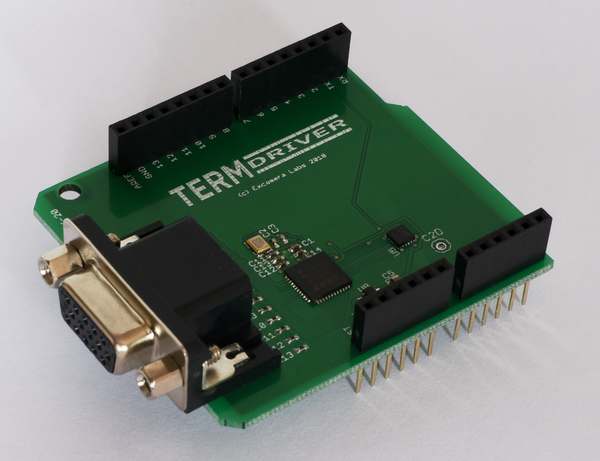
\includegraphics[width=0.75\textwidth]{img/img1}
\end{figure}

TermDriver listens on a serial line and emulates a terminal on a
standard VGA connector. It gives embedded microcontrollers a real
console.

\begin{figure}[H]
  \centering
  \caption{this is an image}
  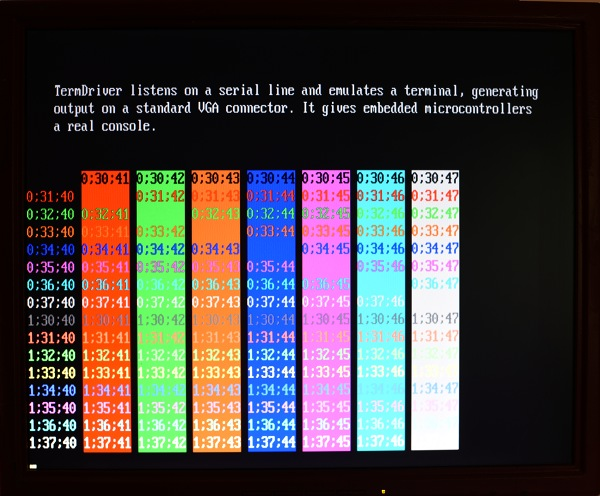
\includegraphics[width=0.75\textwidth]{img/img2}
\end{figure}

TermDriver monitors the serial line at 115200 baud, and any serial
output from the CPU also appears on the VGA. There's nothing to set up
or load. When your microcontroller executes:

\begin{verbatim}
for (;;)
  printf("Counter is %d\n", counter++);
\end{verbatim}

You get this output on the VGA:

\begin{figure}[H]
  \centering
  \caption{this is an image}
  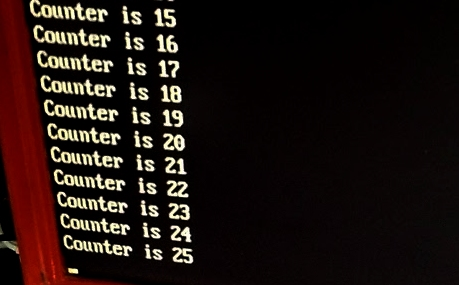
\includegraphics[width=0.75\textwidth]{img/img3}
\end{figure}

It's available in two versions. One has Arduino headers so it's
stackable with any Arduino. The other has no headers, and is meant for
system builders, not necessarily Arduino users.

Hookup is four lines (ground, power, reset, serial) so it's easily
connected to any CPU.

As well as the "classic" 80x25 text mode, the emulation also offers a
higher density 128x48 mode, and a portrait orientation 96x64 mode. Both
are very \href{http://excamera.com/files/DSC_8931.jpg}{readable} because
they match TermDriver's native 1024x768 @ 60 Hz VGA output.

\begin{figure}[H]
  \centering
  \caption{this is an image}
  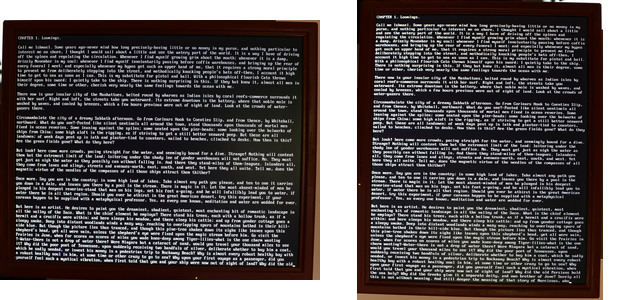
\includegraphics[width=0.75\textwidth]{img/img4}
\end{figure}

The terminal emulation is fully compatible with the DOS
\texttt{ANSI.SYS}, so classic
\href{http://artscene.textfiles.com/ansi/}{ASCII and ANSI art} draws
correctly.

\begin{figure}[H]
  \centering
  \caption{this is an image}
  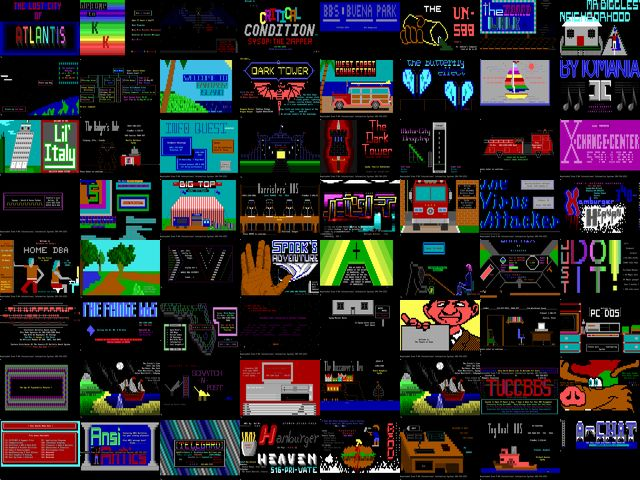
\includegraphics[width=0.75\textwidth]{img/img5}
\end{figure}

\hypertarget{technical-specifications}{}
\hypertarget{technical-specifications}{%
\section{Technical Specifications}\label{technical-specifications}}

The serial line is 115200 baud, 8 bits no parity. The signal level is
3.3 V, and is 5 V tolerant.

Power is 5V. TermDriver has an onboard 3.3 V regulator.

Current consumption is 25 mA when running, 10 mA when in screen saver
mode. The reset signal is active low.

Video output is standard VGA 1024x768 at 60 Hz.

The following standard
\href{https://en.wikipedia.org/wiki/ANSI_escape_code\#CSI_sequences}{CSI
codes} are supported:

\begin{longtable}[]{@{}ll@{}}
\toprule
\begin{minipage}[b]{0.34\columnwidth}\raggedright
Code\strut
\end{minipage} & \begin{minipage}[b]{0.60\columnwidth}\raggedright
Effect\strut
\end{minipage}\tabularnewline
\midrule
\endhead
\begin{minipage}[t]{0.34\columnwidth}\raggedright
ESC {[} \emph{n} A\strut
\end{minipage} & \begin{minipage}[t]{0.60\columnwidth}\raggedright
Cursor up\strut
\end{minipage}\tabularnewline
\begin{minipage}[t]{0.34\columnwidth}\raggedright
ESC {[} \emph{n} B\strut
\end{minipage} & \begin{minipage}[t]{0.60\columnwidth}\raggedright
Cursor down\strut
\end{minipage}\tabularnewline
\begin{minipage}[t]{0.34\columnwidth}\raggedright
ESC {[} \emph{n} C\strut
\end{minipage} & \begin{minipage}[t]{0.60\columnwidth}\raggedright
Cursor forward\strut
\end{minipage}\tabularnewline
\begin{minipage}[t]{0.34\columnwidth}\raggedright
ESC {[} \emph{n} D\strut
\end{minipage} & \begin{minipage}[t]{0.60\columnwidth}\raggedright
Cursor back\strut
\end{minipage}\tabularnewline
\begin{minipage}[t]{0.34\columnwidth}\raggedright
ESC {[} \emph{r;c} H\strut
\end{minipage} & \begin{minipage}[t]{0.60\columnwidth}\raggedright
Cursor position\strut
\end{minipage}\tabularnewline
\begin{minipage}[t]{0.34\columnwidth}\raggedright
ESC {[} \emph{n} J\strut
\end{minipage} & \begin{minipage}[t]{0.60\columnwidth}\raggedright
Erase display\strut
\end{minipage}\tabularnewline
\begin{minipage}[t]{0.34\columnwidth}\raggedright
ESC {[} \emph{n} m\strut
\end{minipage} & \begin{minipage}[t]{0.60\columnwidth}\raggedright
Select graphic rendition\strut
\end{minipage}\tabularnewline
\begin{minipage}[t]{0.34\columnwidth}\raggedright
ESC {[} s\strut
\end{minipage} & \begin{minipage}[t]{0.60\columnwidth}\raggedright
Save cursor position\strut
\end{minipage}\tabularnewline
\begin{minipage}[t]{0.34\columnwidth}\raggedright
ESC {[} u\strut
\end{minipage} & \begin{minipage}[t]{0.60\columnwidth}\raggedright
Restore cursor position\strut
\end{minipage}\tabularnewline
\bottomrule
\caption{this is a table}
\end{longtable}

In addition the following sequences are specific to TermDriver:

\begin{longtable}[]{@{}ll@{}}
\toprule
\begin{minipage}[b]{0.34\columnwidth}\raggedright
Code\strut
\end{minipage} & \begin{minipage}[b]{0.60\columnwidth}\raggedright
Effect\strut
\end{minipage}\tabularnewline
\midrule
\endhead
\begin{minipage}[t]{0.34\columnwidth}\raggedright
ESC {[} \emph{n} h\strut
\end{minipage} & \begin{minipage}[t]{0.60\columnwidth}\raggedright
Set display mode.

0 is 80x25, 1 is 128x48, 2 is 96x64 (rotated)\strut
\end{minipage}\tabularnewline
\begin{minipage}[t]{0.34\columnwidth}\raggedright
ESC {[} \emph{n} S\strut
\end{minipage} & \begin{minipage}[t]{0.60\columnwidth}\raggedright
Screen-saver.

0 stops video output, 1 restarts video output\strut
\end{minipage}\tabularnewline
\bottomrule
\caption{this is a table}
\end{longtable}

\end{document}
